\documentclass{article}
\usepackage[a4paper, total={6in, 9in}]{geometry}
\usepackage[utf8]{inputenc}
\usepackage{graphicx}
\graphicspath{ {./res/} }
\usepackage{float}
\usepackage{listings}
\usepackage{xcolor}
\usepackage{hyperref}
\usepackage{dirtree}
\usepackage{tabularray}

% Colors
\definecolor{strings}{HTML}{448c25}
\definecolor{comments}{HTML}{aaaaaa}
\definecolor{keywords}{HTML}{aa3d8c}
\definecolor{ndkeywords}{rgb}{.612,.36,.15}
\definecolor{background}{HTML}{fbfbfb}
\definecolor{numbers}{HTML}{aaaaaa}

% Listings
% Default style
\lstdefinestyle{default}{
    backgroundcolor=\color{background},
    basicstyle=\ttfamily\small,
    breakatwhitespace=true,
    breaklines=true,
    commentstyle=\color{comments},
    deletekeywords={},
    escapeinside={}{},
    extendedchars=true,
    frame=lines,
    keepspaces=true,
    keywordstyle=\color{keywords},
    keywords={for, in, new, true, false, return, if, while, do },
    ndkeywords={class, export, boolean, void, int, char, throw, include, ifndef, define, endif, private, public, final, this, extends, protected, var},
    ndkeywordstyle=\color{ndkeywords}\bfseries,
    morekeywords={@Override, For, ForEach, Run, Invoke, AsParallel, AsOrdered},
    numbers=none,
    numberstyle=\ttfamily\color{numbers},
    rulecolor=\color{numbers},
    showspaces=false,
    showstringspaces=false,
    showtabs=false,
    stepnumber=1,
    stringstyle=\color{strings},
    morestring=[b]',
    morestring=[b]",
    comment=[l]{//},
    tabsize=2,
}
\lstset{
    style=default,
    columns=fullflexible,
    upquote=true
}

\lstdefinelanguage{numbered}{
    numbers=left,
    numberstyle=\ttfamily\color{numbers},
}

\title{Parallel Programming, FS2023}
\author{Luzia Kündig}
\begin{document}

\maketitle

\section{Week 4 Introduction}

Modern hardware does not run on single cores anymore.

Moores Law: The number of transistors that can be packed into a given unit of space will double about every two years. Which means doubling the speed of a computer every two years.

Physical limits of this law have been reached already. New ways of speeding up processors are needed.

\begin{figure}
    \centering
    \includegraphics*[width=10cm]{res/01-stats.png}
    \caption{CPU Statistics}
\end{figure}

\subsection{Parallelism}
Better CPU utilization, more responsive programs. Divide / modularize tasks of our program. Better software division.

\emph{Hyperthreading}: two register sets to keep two separate contexts. If one task is busy, switch to other context can happen extremely fast. Creates two logical cores from one physical core. More efficient usage of a single hardware construct, use wait time.

Performance increase is \emph{not} 100\% the amount of logical cores.

\subsection{Parallel vs Concurrent}
\emph{Parallel}: different Processors, at the same time. \\
\emph{Concurrent}: Time-shared, switches between two contexts needed. One actor.

After the end of moores law: parallelization is needed for more speedup.

\subsection{OS-Level Parallelism}

\subsubsection{Process vs. Thread}

Process: separates memory completely from other threads. context switches are slow

Threads: Each has their own stack, but all threads inside a process share the same heap. Access to this storage must be synchronized.

\subsubsection{User- vs Kernel Threads}

Only kernel-level threads let you exploit the parallelism speedup on multiple cores.

User-threads (green threads) only live within Application. No true parallelism.

JVM always launches a kernel-level thread.

\subsection{Thread Scheduling}

This is concurrency: Interleaved execution.

Each processor can execute one thread at a time. Multiple Threads are managed via scheduling mechanisms.

States: Running, ready, waiting.

Context switches are "lightweight" but still have a performance impact.

\emph{synchron} (cooperative) waiting for condition, queues itself as waiting
\emph{asynchron} (preemptive) resource are released after a set amount of time

\subsection{JVM Thread Model}

\emph{intra-process communication}

Java Virtual Machine is run as one single process. Main method is called from a startup thread created by the JVM (garbage collectors etc. start their own threads).

JVM process runs as long as all started threads are running. Exception: daemon threads are aborted ad JVM end.

Runtime.Exit()/System.exit() ends jvm abruptly

\subsubsection{Java Threading}

Interface Runnable \\
Class Thread (implements Runnable)

Call Thread(Runnable behaviour);

var myThread = new Thread();

myThread.start();

---

Only guarantee possible: statements inside one thread will always be executed in correct order.

Java important: sth.start() starts a new thread and calls the .run() method. if run() is called by the user, the runnable action will be run sequentially.

\subsubsection{Non-Determinism}
No control: Threads run in any order without any precautionary rules. println in some JVMs is one synchronized (atomar) operation and will not be broken apart. Not always, implementation specific. 

\subsubsection{Variants of Running Threads}

Explicit Runnable Implementation: write named function that implements Runnable Interface.
Sub-Class of Thread: new Class with custom implementation of the run function

\subsubsection{Thread Methods}

\textbf{Thread Join:} \\
t2.join() blocks t1 from running as long as t2 is still running.

\textbf{Thread Sleep:} \\
running thread goes into waiting state until the time has passed for it to be ready again.

\textbf{Thread Yield:} \\
running thread releases the processor but will directly be ready again. not really necessary in time-shared / preemptive scheduling of the scheduler.

\textbf{Thread Interrupt:} \\

\textbf{currentThread:} \\

\textbf{setDaemon:} \\
\section{Week 2 Monitor Synchronization}

Race Condition: 2 Threads try to update the same shared (on heap) resource. 
Outcome: either one of the threads can write, the other update gets lost.

\verb|this.balance += amount| gets converted into three separate instructions. They will not be executed atomically.

Synchronization: restriction of concurrency.

Critical section: only one thread at a time can enter and execute this part of the code.

\subsection*{Synchronized Methods with Monitor}
Java: Keyword \verb|synchronized| in a method header guarantees that the method body is executed atomically.

Every object has a (Monitor-) Lock, which is acquired when any synchronized method is accessed. \verb|static| methods acquire the class objects lock which there is only one of.

Internal mutual exclusion, only one thread operates at a time. all not-private methodsa re synchronized

Wait \& Signal Mechanism: Outer waiting room to acquire Monitor Lock. Inner Waiting Room to wait for condition to be fulfilled.

Two methods: \verb|wait();| for condition, and \verb|notifyAll();| if something in a variable has changed.

Monitor Lock is only freed on method end, not notify/All.

\verb|notifyAll()| if the balance on bank account is increased by a deposit, every withdrawing thread should check their condition again, not just one.. 

\verb|notify()| is enough, if two conditions are fulfilled:\\
\begin{itemize}
    \item Uniform waiting condition (boolean): a change in the condition interests every waiting thread 
    \item One in one out: only a single waiting thread can continue
\end{itemize}

while loop: Check should happen every time the thread has access to the Monitor, not just the first time. Thread execution continues from where it has left off.

Spurious Wakeup: thread wakes up out of a special reason, maybe woken by the OS.

\subsection{Discussion}

Advantage: very powerful concept, object oriented\\

\noindent
Disadvantage: not always optimal. efficiency and fairness problems
\section{Synchronization Primitives}

\subsection{Semaphores}

Is in essence a counter which defines the number of free resources, coupled with operations to adjust that record \emph{safely}.

\texttt{new Semaphore(number);}

General Semaphore (0-n) vs. Binary Semaphore (Mutex, 0 or 1). Fairness can be enforced using FIFO waiting queue, slower than non-fair version:

\texttt{new Semaphore(number, true);}

\begin{description}
  \item[acquire()] acquire a permit, decrement counter of available resources. Wait if none is available. Thread is disabled for scheduling and lies dormant until it can acquire the semaphore or is interrupted.
  \item[release()] free a permit, increment counter of available resources, notifies waiting threads. \textit{does not confirm that acquire() has been called before.}
\end{description}

\subsubsection*{Implementation using Monitor}
\begin{verbatim}
  public class Semaphore {
    private int value;

    public Semaphore(int initial) {
      value = initial;
    }
    public synchronized void acquire() throws InterruptedException {
      while (value <= 0) { wait(); }
      value--;
    }
    public synchronized void release() {
      value++;
      notify();
    }
  }
\end{verbatim}

\subsection{Lock and Condition}

Uses a \texttt{ReentrantLock}, which is \textit{owned} by the thread that last successfully locked and not yet unlocked it. Always follow a successful \texttt{lock} with a \texttt{try / finally} block to ensure it is unlocked in case of an exception.

\texttt{Conditions} can be created from an existing ReentrantLock.

\begin{verbatim}
  private Lock monitor = new ReentrantLock(true);
  private Condition nonFull = monitor.newCondition();
  private Condition nonEmpty = monitor.newCondition();

  public void put(T item) throws InterruptedException {
    monitor.lock();
    try {
      while (queue.size() == Capacity) { nonFull.await(); }
      queue.add(item);
      nonEmpty.signal();
    } finally { monitor.release(); }
  }
\end{verbatim}

\subsection{Read/Write Locks}

Goal: allow parallel read access but mutually exclusive write access.

\begin{verbatim}
  ReadWriteLock rwLock = new ReentrantReadWriteLock(true);
  rwLock.readLock().lock();
  // read only access
  rwLock.readLock().unlock();

  rwLock.writeLock().lock();
  // write and read access
  rwLock.writeLock().unlock();
\end{verbatim}

\subsection{Count Down Latch}
Car Race example:

\begin{verbatim}
  var ready = new CountDownLatch(10); // number of cars
  var start = new CountDownLatch(1);  // start signal given once

  //car
  ready.countDown(); // register for race
  start.await();     // wait for start

  //race control
  ready.await();      // wait until all cars are ready
  start.countDown();  // start signal
\end{verbatim}

\subsection{Cyclic Barrier}

Reusable synchronization point for a given amount of threads that wait.

\begin{verbatim}
  var start = new CyclicBarrier(10); // number of cars
  
  // car
  start.await(); // wait for everyone to be ready
\end{verbatim}

\subsection{Exchanger}
Call blocks until another thread also calls exchange, returns argument of the other thread.

\begin{verbatim}
  var exchanger = new Exchanger<Integer>();
  int out = exchanger.exchange(in);
\end{verbatim}
\section{Week 4 Dangers of Concurrency}

Concurrent programming creates the possibility for new kinds of errors.

\subsection{Parallelism Correctness Criteria}

\begin{description}
  \item[Race Condition] not enough synchronization, possibility of errors that should not happen according to the program logic. Knowledge of 'what is correct' is necessary to specify the error.
  \item[Data Race] actual occurence of an 'illegal' operation on memory in a concurrent context. Several threads access the same variable/array in memory, at least one write acceess, without synchronization. Forbidden in Java Spec, results undefined.
  \item[Deadlock] If two threads wait for each other when trying to lock 2 resources in reverse order. Can be identified with a resource graph. 
  \begin{figure}
    \centering
    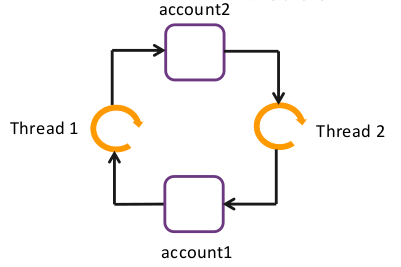
\includegraphics[width=6cm]{res/04-resource-graph.png}
    \caption{Resource Graph identifies Deadlocks}
  \end{figure}
  \textit{Solution:} define an order for locking OR use more coarse granular locking when ordering does not make sense.
  \item[Livelock] Same as deadlock, but executing instructions while waiting. 
  \item[Starvation] When no fairness is in place, one thread runs the risk of having to wait 'forever' to access a resource.
\end{description}

\noindent
\textit{Ergo:} For a program to be formally correct in a parallel execution it must have \textbf{no race conditions, no deadlocks and no starvation.}

\begin{figure}
  \centering
  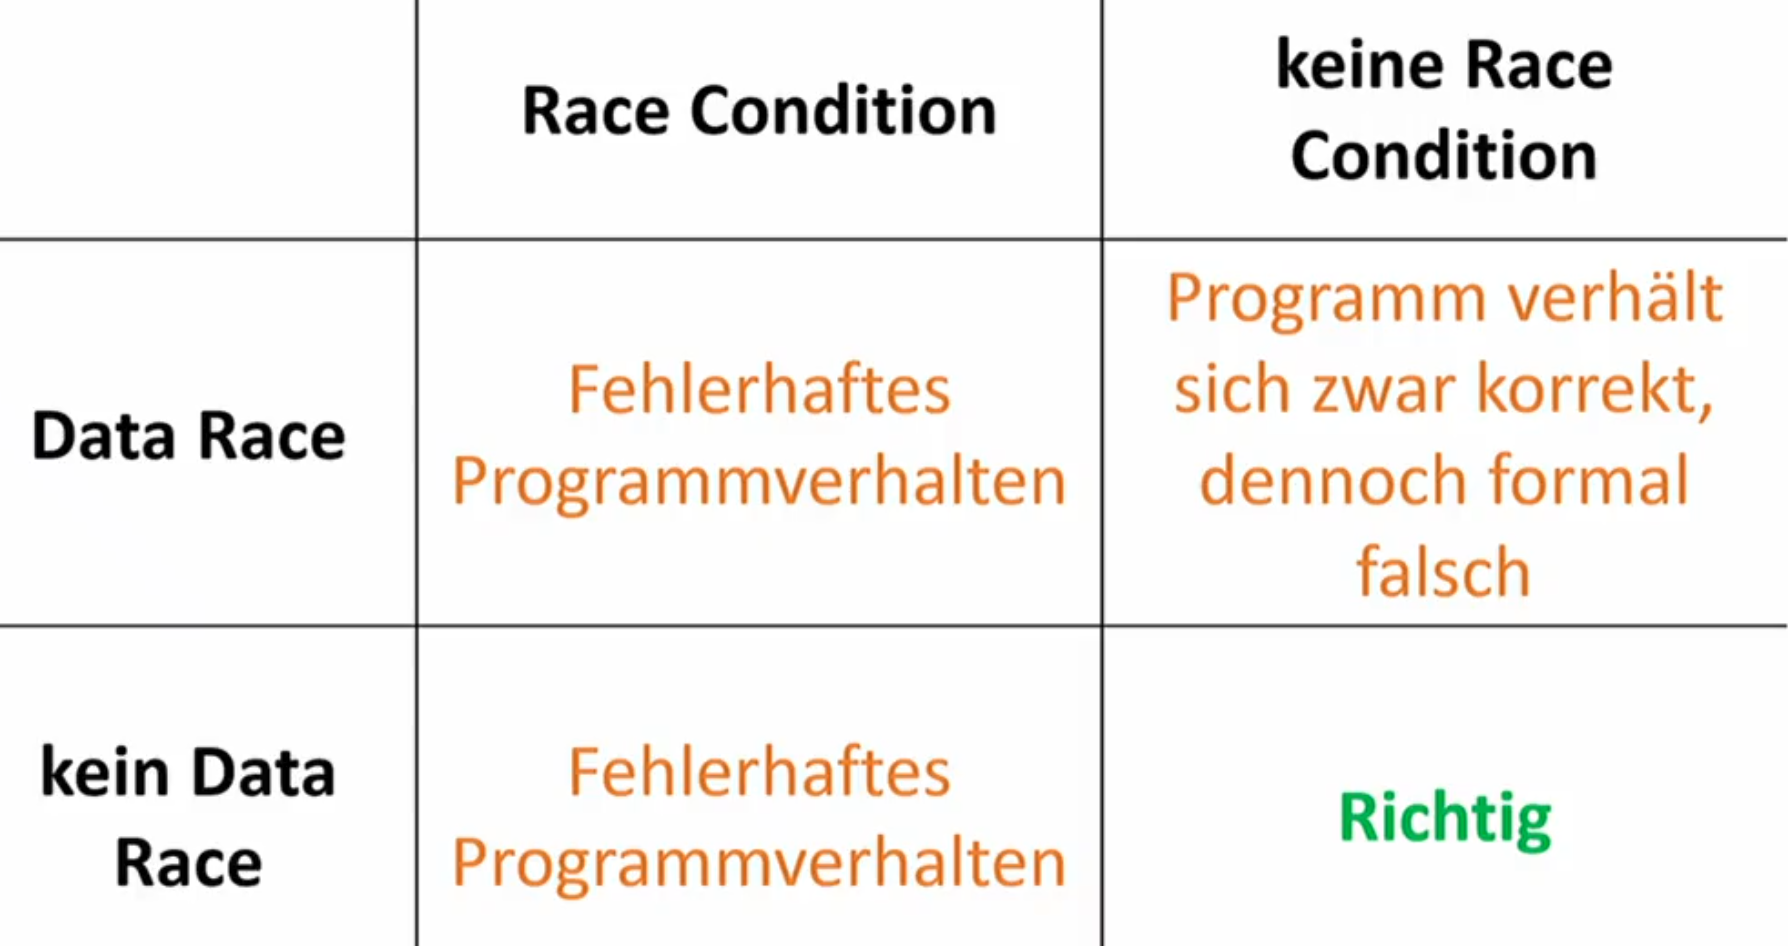
\includegraphics[width=8cm]{res/04-datarace-raceconditions.png}
  \caption{Data Races and Race Conditions}
\end{figure}

\subsection{No Synchronization needed}
\begin{description}
  \item[Immutability] Read only variables
  \item[Thread Confinement] Object belongs to one thread only at any point in time.
  \item[Object Confinement] encapsulation of inner objects by synchronizing all access via an outer class. 
\end{description}

\subsection{Thread Safety}
The avoidance of data races. \textit{When no sharing is intended}, give each thread a private copy of the relevant data.
\textit{When sharing is important}, provide explicit synchronization to make certain the program behaves in a deterministic manner.

\begin{figure}[H]
  \centering
  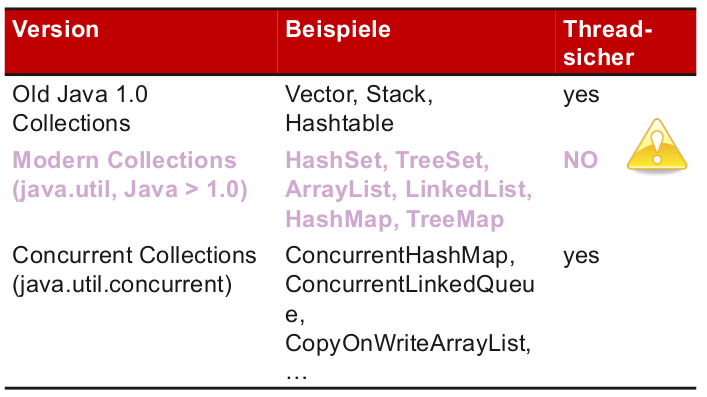
\includegraphics[width=8cm]{res/04-thread-safe-collections.png}
  \caption{Java Collections}
\end{figure}

New approach: provide synchronization only when explicitly needed.

\section{Thread Pools}

Downsides of using many threads include
\begin{itemize}
    \item longer time intervals before the same thread is scheduled again
    \item start and termination of threads has some overhead
    \item number of possible threads is limited
    \item Memory cost: Single stack for each thread
    \item full register-backup at preemption
\end{itemize}

A possible solution strategy is to allow for high parallelism in the problem space, but use a limited number of threads (\# threads \texttt{<=} \# processors).

\begin{description}
  \item[Tasks] define potentially parallel work packages that are \textit{independent} of each other.  
  \item[Task pool] Tasks are queued and executed by different worker threads. The number can be adapted to the system. Any task must complete execution before its worker thread can start another task.
  \textit{Programs that are modeled using tasks will automatically run aster on parallel machines.}
  \item[Return Values] from tasks are packaged into their own object type. \texttt{Future} in Java, \texttt{Promise} in JavaScript, \texttt{Task} in .NET, will return the result once it is available.
  
  Starting a task returns a future value that can be waited on using a method call.
  \item[Worker Threads] are usually daemon threads in TPL and ForkJoinPool: application can stop before the tasks end.
\end{description}

Submitting a task into the pool will launch the task asynchronously. Accessing the result from a future value will block until the task is terminated.

\subsection{Java Fork Join Pool}

Use \texttt{submit()} for asynchronous execution, \texttt{invoke()} for blocking execution.

\begin{lstlisting}
  var threadPool = new ForkJoinPool(); // create new pool
  var default = ForkJoinPool.commonPool(); // default pool as singleton
  
  Future<Integer> future = threadPool.submit(() => {
    int value = ...; // some long calculation
    return value;
    })

    int result = future.get(); // blocking call
  \end{lstlisting}
  
  \begin{figure}
    \centering
    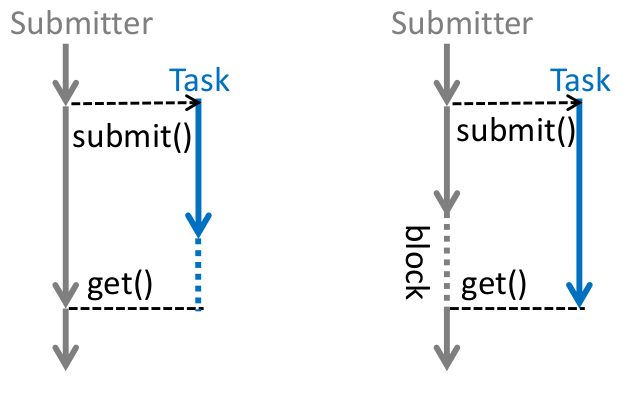
\includegraphics[width=6cm]{res/05-future.png}
    \caption{Future}
  \end{figure}

  \begin{description}
    \item[RecursiveAction] for tasks without return value (= \texttt{RecursiveTask<Void>})
    \item[invokeAll()] to start and wait for sub-tasks
  \end{description}

\subsection{.NET TPL: Task Parallel Library}
Has multiple abstraction layers:
\begin{itemize}
  \item Task Parallelization: use tasks explicitly
  \item Data Parallelization: use parallel statements and queries (implicit tasks)
  \item Asynchronous Programming (async/await)
\end{itemize}

\begin{description}
  \item[Exception in threads] terminates the program.
  \item[Fairness flag] not available.
  \item[Lock\&Condition] not available.
  \item[ReadWriteLockSlim] for upgradeable Read/Write Lock.
  \item[Semaphores] can be used at OS level.
  \item[Mutex] binary semaphore at OS level
  \item[Collections] are not thread safe, except \texttt{System.Collections.Concurrent} 
\end{description}

\begin{lstlisting}
  Task task = Task.Run(() => {
    // task implementation
  });
  // other code
  task.Wait(); // blocking call for task without return value
  Console.Write(task.Result); // blocking call, returns result
\end{lstlisting}

Nested tasks are possible:

\begin{lstlisting}
  var task = Task.Run(() => {
    var left = Task.Run(() => Count(leftPart));
    var right = Task.Run(() => Count(rightPart));
    return left.Result + right.Result;
  });
\end{lstlisting}

Using implicit Tasks, wait barrier at the end: \begin{lstlisting}
  Parallel.Invoke(
    () => MergeSort(l, m),
    () => MergeSort(m, r)
  );
\end{lstlisting}

Data Parallel for each:
\begin{lstlisting}
  Parallel.ForEach(list, 
    file => Convert(file)
  );
\end{lstlisting}


Data Parallel for (when iterations are independent):
\begin{lstlisting}
  Parallel.For(0, array.Length, 
    i => DoComputation(array[i])
  );
\end{lstlisting}

Parallel Loops will automatically group multiple iterations into one single task to avoid too much overhead.

\subsection{Parallel LINQ}

\begin{lstlisting}
  from book in bookCollection.AsParallel().AsOrdered()
    where book.Title.Contains("Concurrency")
    select book.ISBN
\end{lstlisting}

\subsection{Work Stealing}
In a work stealing scheduler, each processor in a computer system has a queue of work items (computational tasks, threads) to perform. 
Each work item consists of a series of instructions, to be executed sequentially, but in the course of its execution, a work item may also spawn new work items that can feasibly be executed in parallel with its other work. 
These new items are initially put on the queue of the processor executing the work item. 
When a processor runs out of work, it looks at the queues of the other processors and "steals" their work items. 
In effect, work stealing distributes the scheduling work over idle processors, and as long as all processors have work to do, no scheduling overhead occurs \href{https://en.wikipedia.org/wiki/Work\_stealing}{[1]}.
\section{Asynchronous Programming}

\begin{description}
  \item[Task Continuations / CompletableFuture] can create chains of tasks that depend on each other. Wait at the end contradicts the idea, only necessary in special cases (keep main thread running for examples..).
  
  .NET: \texttt{task1
  .ContinueWith(task2)
  .ContinueWith(task3)
  .Wait();} 

  \texttt{Task.WhenAll(task1, task2).ContinueWith(task3);
  Task.WhenAny(task1, task2).ContinueWith(task3);}
  
  Java: \texttt{CompletableFuture
  .supplyAsync(() => firstOp)
  .thenApplyAsync(second)
  .thenAcceptAsync(third)};

  \texttt{CompletableFuture.allOf(future1, future2);
  CompletableFuture.any(future1, future2);}

  Use \texttt{exceptionally()} as Exception-Handling-Continuation
  \begin{figure}[H]
      \centering
      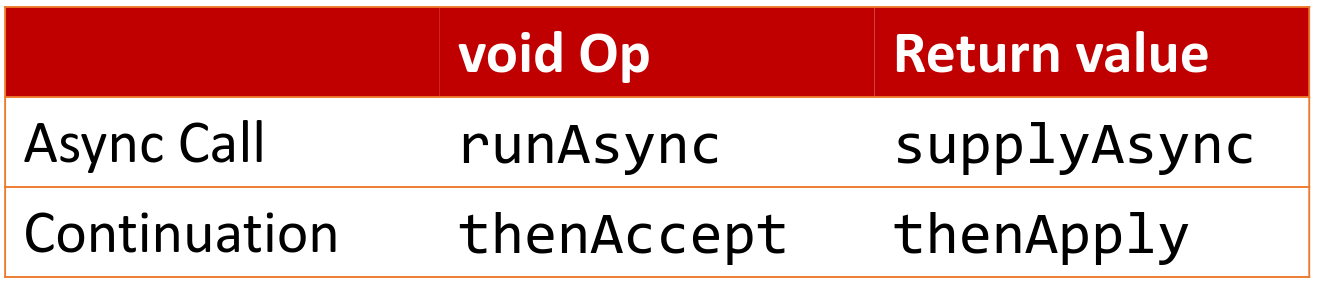
\includegraphics[width=10cm]{res/completable-future.png}
  \end{figure}
  
  \item[Caller-centric vs. Callee-centric] pull: caller requests result, push: callee (task) informs or continues once the result is available.
  
  \item[Exceptions] in Worker Tasks that are never awaited are ignored, in Java and .NET. No way of handling the exception is present. \texttt{TaskScheduler.UnobservedTaskException} could be used, but timing is GC-dependent.
  
  \item[Exceptionally] can be used in Java, similar to finally for try-catch.
\end{description}


\subsection{UI Programming}

Only a single UI Thread is allowed to do operations on UI components. The same thread should not execute long running operations, else the UI becomes unresponsive.

\begin{figure}[H]
  \centering
  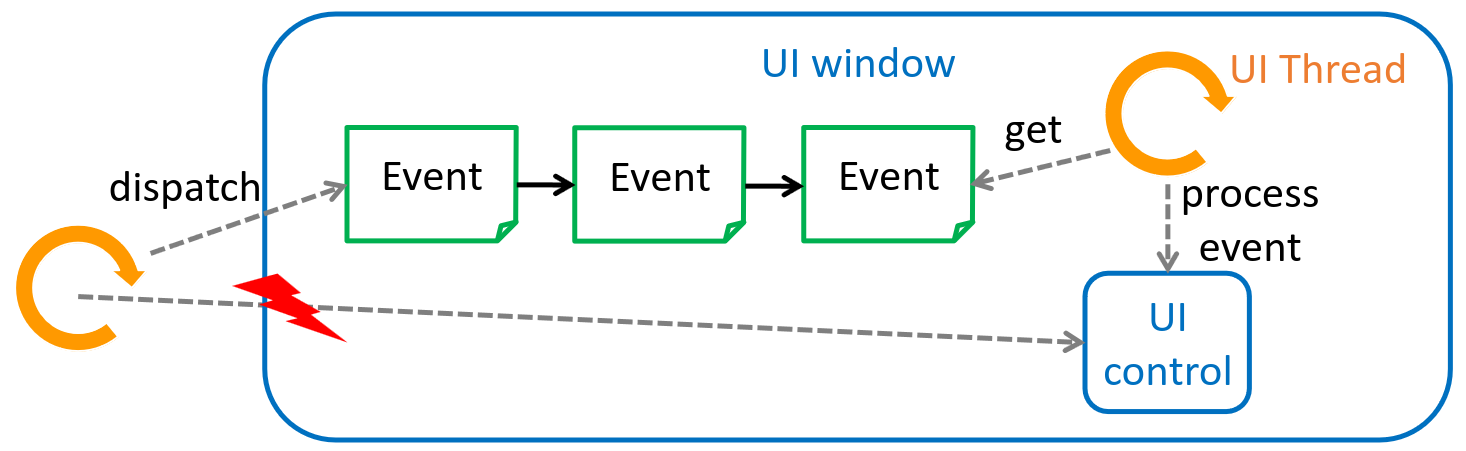
\includegraphics[width=12cm]{res/06-ui-thread-loop.png}
  \caption{UI Thread runs in a loop to process events}
\end{figure}

Logic in Java
\begin{lstlisting}
  button.addActionListener(event ->
    var url = textField.getText();
    CompletableFuture.runAsync(() -> {
      var text = download(url);
      SwingUtilities.invokeLater(() -> {
        textArea.setText(text);
      });
    });
  );
\end{lstlisting}

Logic in .NET
\begin{lstlisting}
  void buttonClick(...) {
    var url = textBox.Text;
    Task.Run(() => {
      var text = Download(url);
      Dispatcher.InvokeAsync(() -> {
        label.Content = text;
      });
    });
  }
\end{lstlisting}

Logic in .NET with async/await
\begin{lstlisting}
  var url = textBox.Text;
  var text = await DownloadAsync(url); // executes on worker thread
  label.Context = text;
\end{lstlisting}

Asynchronous methods are split up by the compiler. First part is run synchronously, code after the blocking call may be executed by another thread as a continuation.
If caller is a "normal" thread, execution is dispatched to another TPL worker thread. 
If caller is a UI thread, continuation is dispatched and processed as a UI event.

\subsection*{Async return value types}
\texttt{void}: fire and forget. 
\texttt{Task}: allows waiting for completion. 
\texttt{Task<T>}: allows waiting for a result of type T.
No support for \texttt{ref} or \texttt{out} parameters.

\vspace{3mm}
Async method must use await statement, else compiler will warn. Use tasks if necessary. Example:

\begin{lstlisting}
  public async Task<bool> IsPrimeAsync(long number) {
    return await Task.Run(() => {
      for (long i = 2; i * i <= number; i++) {
        if (number % i == 0) { return false; }
      }
      return true;
    });
  }
\end{lstlisting}
\section{Week 7 Memory Models}

\subsection{Problem Causes}

\subsection{Atomicity}

\subsubsection*{Atomic Base Types (Boolean, Integer, Long, Reference)}

\subsubsection*{getAndSet}
\verb|boolean locked|

\verb|locked.getAndSet(true)| always returns the initial value read.

\verb|while(locked.getAndSet(true)) {}| loops until the value of locked is false.

\subsubsection*{CompareAndSet}

\subsubsection{Optimistic Synchronization}
\begin{verbatim}
    do {
        oldValue = var.get();
        newValue = calculateChanges(oldValue);
    } while (!var.compareAndSet(oldValue, newValue));
\end{verbatim}

\subsubsection*{CompareAndExchange}
like compare and set, returns current in any case

\subsubsection*{updateAndGet}


\subsection{Visibility}

\subsection{Ordering}
\section{Exercise 1}

\begin{itemize}
  \item "normal" Tread vs. Daemon Thread
  \item find number of cores on a machine
  \item find the maximum number of threads that can run in a java program: limit is memory.. stack is allocated for each process
\end{itemize}

% \dirtree{%
%   .1 init/.
%   .2 definitions/.
%   .3 index/.
%   .4 mapping/.
%   .5 assignment.json.
%   .5 comment.json.
%   .5 testresult.json.
%   .4 settings/.
%   .5 testresult.json.
%   .3 pipelines/.
%   .4 testresult.json.
%   .2 search-templates/.
%   .3 get-all-hosts.json.
%   .3 get-branch-names.json.
%   .3 get-by-start-time.json.
%   .3 get-comments.json.
%   .3 get-commit-history.json.
%   .3 get-dashboard.json.
%   .3 get-distinct.json.
%   .3 get-errors-by-host.json.
%   .3 get-oldest-date.json.
%   .3 get-regression.json.
%   .3 get-test-environment-history.json.
%   .3 get-testsuite-aggregation.json.
%   .3 get-with-should-filter.json.
%   .2 Dockerfile.
%   .2 init.sh.
% }

\subsection*{Parallel Counting}
\begin{lstlisting}
  var left = threadPool.submit(() => count(leftPart));
  var right = threadPool.submit(() => count(rightPart));
  result = left.get() + right.get();
\end{lstlisting}

\subsection*{Recursive Counting}
\begin{lstlisting}
  class CountTask extends RecursiveTask<Integer> {
    // constructor

    @Override
    protected Integer compute() {
      // if no or single element, return result
      // split into two parts
      var left = new CountTask(lower, middle),
      var right = new CountTask(middle, upper);
      left.fork(); right.fork();
      return right.join() + left.join();
    }
  }
\end{lstlisting}

\subsection*{Full Task Implementation}
\begin{lstlisting}
  class CountTask extends RecursiveTask<Integer> {
    private final int lower, upper, THRESHOLD; // threshold to avoid over-parallelization
    public CountTask(int lower, int upper) {
      this.lower = lower; this.upper = upper;
    }
    protected Integer compute() {
      if (lower == upper) { return 0; }
      if (upper - lower < THRESHOLD) { 
        // sequential execution
        return isPrime(lower) ? 1 : 0; 
        }
      // parallel execution
      int middle = (lower + upper) / 2;
      var left = new CountTask(lower, middle);
      var right = new CountTask(middle, upper);
      left.fork(); right.fork();
      return right.join() + left.join();
    }
  }
\end{lstlisting}

\end{document}